\documentclass[sigconf]{acmart}

\usepackage{booktabs} % For formal tables
\usepackage{hyperref}
\usepackage{listings}
\usepackage{graphicx}


% Copyright
%\setcopyright{none}
%\setcopyright{acmcopyright}
%\setcopyright{acmlicensed}
\setcopyright{rightsretained}
%\setcopyright{usgov}
%\setcopyright{usgovmixed}
%\setcopyright{cagov}
%\setcopyright{cagovmixed}


% DOI
% \acmDOI{10.475/123_4}

% ISBN
% \acmISBN{123-4567-24-567/08/06}

%Conference
\acmConference[UPDS-SoSe18]{Uni Passau - Data Science Seminar - SoSe18}{July 2018}{Passau, Germany}
\copyrightyear{2018}

\begin{document}
\title{Hyperparameter Study for Classical Feed-forward Neural Networks on Text Data}

\author{Marius Kleidl}
\affiliation{%
  \institution{University of Passau}
  \city{Passau}
}
\email{kleidl01@gw.uni-passau.de}

\begin{abstract}
	In this paper we train and evaluate the accuracy of text classifiers using simple feed-forward neural networks with different learning rates, numbers of hidden layers and numbers of perceptrons per layer. Our results show that different values for these hyperparameters influence the classifier's accuracy while their impact on the performance is limited. We conclude that better text preprocessing and feature selection steps may be necessary to further improve the classifier. As we choose general-purpose hyperparameters for the experiment, the impact of this paper should not be neglected, even if the results are not comparable with state-of-the-art techniques.
\end{abstract}

%
% The code below should be generated by the tool at
% http://dl.acm.org/ccs.cfm
% Please copy and paste the code instead of the example below.
%
\begin{CCSXML}
	<ccs2012>
	<concept>
	<concept_id>10010147.10010257.10010258.10010259.10010263</concept_id>
	<concept_desc>Computing methodologies~Supervised learning by classification</concept_desc>
	<concept_significance>500</concept_significance>
	</concept>
	<concept>
	<concept_id>10010147.10010257.10010293.10010294</concept_id>
	<concept_desc>Computing methodologies~Neural networks</concept_desc>
	<concept_significance>500</concept_significance>
	</concept>
	</ccs2012>
\end{CCSXML}

\ccsdesc[500]{Computing methodologies~Supervised learning by classification}
\ccsdesc[500]{Computing methodologies~Neural networks}

\keywords{Machine Learning, Text Classification, Neural Networks}

\maketitle

\section{Introduction}

In Natural Language Processing applications the task of classifying text is a common one and is widely used in areas such as sentiment analysis, recommendation engines and content filtering. Neural networks have received increasing attention for solving these complex problems and have achieve impressive results. However, as with any machine learning application it is necessary to properly adjust the network's hyperparameters to the specific use case and its data set. This optimization process can be a though challenge which is often solved by simple trial and error.

In our contribution we provide an experiment showing the challenge of this process. We train a feed-forward neural network on text classification using different hidden layers and learning rates. After in in-depth description of our experiment, we present the results and discuss the limited impact of the two chosen hyperparameters on the classifier's accuracy.

Even if our results are not comparable to the ones of other state-of-the-art approaches, the impact of this paper cannot be neglected as choosing the most suitable values for the basic hyperparameters forms an important foundation for further optimizations of the network.

\section{Background}

Feed-forward neural networks consist of multiple layers. Each layer contains a varying number of perceptrons where each perceptron is connected to all perceptrons of the next layer\cite{nielsenneural}. As Figure~\ref{fig:layers} shows, a network has a single input layer, one or mode hidden layers and again one output layer. In feed-forward neural networks signals will only travel in one direction, flowing from one layer to the next layer, as illustrated by the arrows in Figure~\ref{fig:layers}. Furthermore, only direct connections to the next layers are allowed, preventing circles as used in recurrent neural networks. 

\begin{figure}
	\centering
	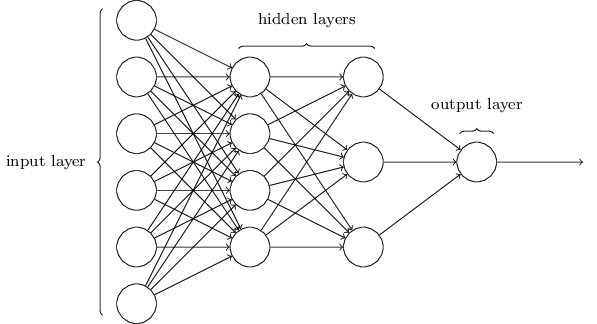
\includegraphics[width=8cm]{layers.png}
	\caption{Layout of a feed-forward neural network with one input layer, two hidden layers and a single output layer. Each layer has a different number of perceptrons illustrated by the circles. Source: \href{http://neuralnetworksanddeeplearning.com/chap1.html}{http://neuralnetworksanddeeplearning.com/}}
	\label{fig:layers}
\end{figure}

Text classification is the process of assigning a class to a provided text phrase. In this paper we will focus on multi-class classification meaning that the classifier has to choose one out of more than two classes\footnote{In contrast, if only two classes are provided, it's called binary classification.}. In our data set 20 classes are available, as will be described in section \ref{text-data-set}. Only one class will be assigned to a text phrase in our experiment.

\section{Contribution}

In our experiment we train and evaluate the performance of multiple deep neural networks with different numbers of layers, numbers of perceptrons per layer and different learning rates.
This section describes the setup of our experiment, in particular the data set, the chosen feature extraction steps, the hyperparameters for our neural network and our evaluation method. The experiment is conducted using the machine learning software scikit-learn\cite{scikit-learn} in its version 0.19.1.
The source code for this experiment is available at the public repository\cite{exp-code} for reproduction.

\subsection{Text Data Set}
\label{text-data-set}

The experiments are performed using the well-known 20Newsgroups\footnote{\href{http://qwone.com/~jason/20Newsgroups/}{http://qwone.com/$\sim$jason/20Newsgroups/}} data set. It contains 18846 postings in the English language which are nearly evenly distributed across 20 different newsgroups, as can be seen in Table~\ref{tab:groups}. Furthermore, the set has been split into a training set of 11314 posts and a testing set of 7532 posts. Posts have been put into one of the two sets based on whether they have been created before or after a specific date\cite{sklearn-newsgroup}.

An example for a post's format is given in Figure~\ref{fig:post}. As one can see, the post contains a header and a signature section consisting of additional meta data, such as the sender's e-mail address and organization. To prevent our neural network from associating this meta data with specific classes, we remove the headers and signatures from each post.

\begin{figure*}
	\begin{center}
		\begin{tabular}{c}
			\begin{lstlisting}[basicstyle=\footnotesize]
From: JC924@uacsc2.albany.edu
Subject: Why are our desktop fonts changing?
Organization: University at Albany, Albany NY 12222
X-Newsreader: NNR/VM S_1.3.2
Lines: 17

One of our users is having an unusual problem.  If she does an Alt/Tab to
a full-screen DOS program, when she goes back to Windows her desktop fonts
have changed.  If she goes back to a full-screen DOS program and then goes
back to Windows, the font has changed back to its default font.  It's not
a major problem (everything works and the font is legible), but it is
annoying.  Does anyone have any idea why this happens.  By the way, she
has a DEC 486D2LP machine.


++++++++++++++++++++++++++++++++++++++++++++++++++++++++++++++++++++++++++
Jeffrey M. Cohen                      Voice: 518-442-3510
Office for Research (AD 218)          Fax:   518-442-3560
The University at Albany              E-mail: JC924@uacsc2.albany.edu
State University of New York
1400 Washington Ave.
Albany, NY 12222
++++++++++++++++++++++++++++++++++++++++++++++++++++++++++++++++++++++++++++
			\end{lstlisting}
		\end{tabular}
	\end{center}
	\caption{Post example from the comp.os.ms-windows.misc newsgroup}
	\label{fig:post}
\end{figure*}

\begin{table}[]
	\centering
	\caption{Posts per newsgroup}
	\label{tab:groups}
	\begin{tabular}{c|c}
		\hline
		       Newsgroup         & Number of posts \\ \hline
		    rec.motorcycles      &       996       \\
		 comp.sys.mac.hardware   &       963       \\
		   talk.politics.misc    &       775       \\
		 soc.religion.christian  &       997       \\
		     comp.graphics       &       973       \\
		        sci.med          &       990       \\
		   talk.religion.misc    &       628       \\
		     comp.windows.x      &       988       \\
		comp.sys.ibm.pc.hardware &       982       \\
		   talk.politics.guns    &       910       \\
		      alt.atheism        &       799       \\
		comp.os.ms-windows.misc  &       985       \\
		       sci.crypt         &       991       \\
		       sci.space         &       987       \\
		      misc.forsale       &       975       \\
		    rec.sport.hockey     &       999       \\
		   rec.sport.baseball    &       994       \\
		    sci.electronics      &       984       \\
		       rec.autos         &       990       \\
		 talk.politics.mideast   &       940
	\end{tabular}
\end{table}

\subsection{Feature Extraction of Text Data}
\label{sec:feature}

Since raw sequences of characters cannot be processed by neural networks, we need to represent our data in vectors of fixed size. In order to achieve this, the text has been converted into the commonly used bag-of-words model after removing English stop words, such as "the" and "is". Our model only contains single words and not pairs of words\footnote{These pairs of words are commonly known as bigrams and are used to keep information about the structure of sentences.}. Furthermore, the model does not discard words depending on their frequency of occurrence. Every word used in the text is included in the model, even if it only appears once\footnote{Another experiment we conducted showed that removing less commonly used words reduces the number of features but does not improve the accuracy. Since this is out of this paper's scope, it will not be described in more detail in this paper.}.

Next, we normalize the entries in our bag-of-words representation. For classification words with a higher frequency of occurrence are usually less informative than specialized words which are more rarely used. For example, from the word "time" we cannot infer a possible topic since it can be used in a variety of contexts. On the other hand, the specialized word "alternator" is rarely used but if so, it may likely be in the context of automobiles.

Therefore, if we would use the frequency of occurrence for rating a word's importance, we will assign more specialized words a less important impact. This low rating causes that specialized words are considered as of less importance than general words, even though it's the opposite. To avoid this, we need to prevent that a word's importance is based on its frequency of occurrence. This can be achieved by rating a word's impact based on its term frequency-inverse document frequency (TFIDF). Using this normalization, words with a high frequency will by considered of less importance.

\subsection{Deep Neural Network for Classification}
\label{deep-neural-network}

Our neural networks contain one or two hidden feed-forward layers consisting of 50 or 100 perceptrons. The learning rate is 1, 0.1, 0.01, 0.001 or 0.0001. For the activation function we choose the rectified linear unit function (ReLu) as defined by $f(x) = max(0, x)$. This decision was based on previous work which showed that the ReLu is able to provide better classification accuracy in supervised training than the hyperbolic tan function or the the logistic sigmoid function\cite{pmlr-v15-glorot11a}. The loss-function is optimized using the stochastic gradient descent optimizer Adam as proposed by Kingma, Diederik, and Jimmy Ba\cite{adam}. The L2 penalty parameter $alpha$ for regularization has been set to 0.0001.

Each neural network is trained until its accuracy stops to increase noticeably. For this purpose, 10\% of the training set will be randomly split apart as a validation set. After each training iteration using the remaining 90\% the network's performance will be evaluated using the validation set. If the mean accuracy across all classes does not improve more than 0.1 percentage point for two iterations, the training will be stopped. 

\subsection{Evaluation}

The classifier's performance is measured using its mean accuracy. This score is defined as the mean of the classifier's accuracy for each label.

In order to find the best combination of hidden layers and learning rate, we perform a grid search where for each combination of these parameters a classifier is trained and evaluated using the mean accuracy. As mentioned above, our learning rate is one of 1, 0.1, 0.01, 0.001 and 0.0001 while the number of layers is one or two with 50 or 100 perceptrons per layer. In total we train and evaluate the performance of 20 neural networks.

To further ensure that we do not overfit our model on our test data set, we are using 4-folded cross validation. In this method, the training set for a classifier will be split into four distinct folds. Next, four sub-classifiers will be trained using three of the four distinct folds and one fold will be used for validation. For each sub-classifier the validation set will be a different one. Finally, the mean value of the four sub-classifiers' accuracies is calculated which is then in turn used as the accuracy for the entire classifier\cite{introduction_ml}.

\section{Results}

\begin{figure}
	\centering
	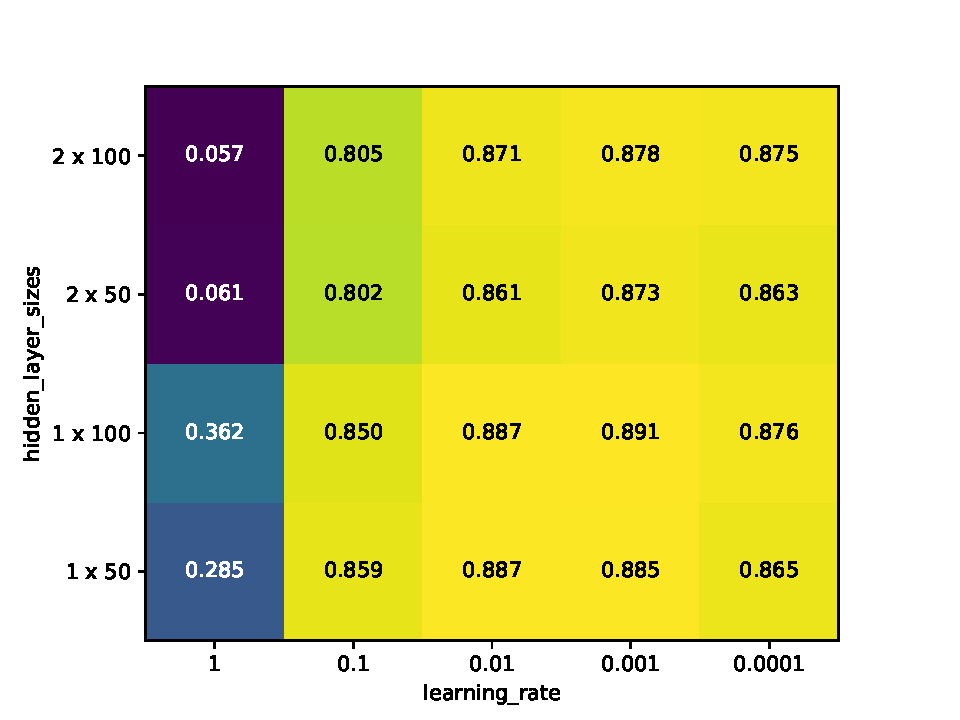
\includegraphics[width=9cm]{fig2.pdf}
	\caption{Mean training accuracy for classifiers using different hyperparameters. The X-axis depicts te learning rate while the Y-axis show the number of hidden layers and number of perceptrons per hidden layer.}
	\label{fig:heatmap}
\end{figure}


Figure~\ref{fig:heatmap} shows the mean accuracy of the classifiers which were trained using the different hyperparameters values. We can see that the neural network with one hidden layer of 100 perceptrons and a learning rate of 0.001 performed the best out of our evaluated classifiers. It achieved a mean accuracy of about 89.1\% during training. 

In order to evaluate the actual accuracy of the best classifier in real-world situations, we let the neural network predict the newsgroups for the separate testing data set of 7532 posts. Since this data set has not been used for training or validation of the classifiers, it is a good fit for evaluating the actual accuracy. The classifier with one hidden layer of 100 perceptrons and a learning rate of 0.001 is able to achieve a \textbf{mean accuracy} of 81.5\%. The \textbf{macro F1 score} is 80.8\% and the \textbf{micro F1 score} is 81.5\%.

The difference between the reported accuracy during training and the actual accuracy using the unseen testing data set is 7.6 percentage points. This number is significant yet expected, as we indirectly chose the classifier which performs best on the training set. A good performance on the training set does not imply an equally good performance on the unseen testing set.

Furthermore, Figure~\ref{fig:heatmap} reveals that the classifiers using one hidden layer with 50 or 100 perceptrons and a learning rate of 0.01 were able to achieve a mean accuracy of about 88.7\% each, which is only off by 0.4 percentage points from out best classifier. The classifier using one hidden layer of 50 perceptrons and a learning rate of 0.001 was less effective with a mean accuracy of 88.5\% which results in a difference of 0.6 percentage points from our best classifier.

A more significant difference can be seen when looking at the neural networks with multiple hidden layers. There, the neural network with two hidden layers of 50 perceptrons and a learning rate of 0.1 achieve only a mean accuracy of 80.2\%.
Also notably, the neural networks with a learning rate of 1 achieved a maximum mean accuracy of 36.2\%, which is expect as such a high value hinders the optimization of the loss function.

\section{Discussion}

From the data presented in Figure~\ref{fig:heatmap}, we can see that the choice of hidden layers and learning rate makes a significant impact on the classifier's accuracy. For example, let's compare two neural networks: On one hand, the neural network consisting of two layers of 50 perceptrons and trained with a learning rate of 0.1 resulted in an accuracy of 80.2\%. On the other hand, the neural network consisting of one layer of 100 perceptrons and trained with a learning rate of 0.001 resulted in an accuracy of 89.1\%. The difference in their accuracies is 8.9 percentage point which is a significant number.
However, we also see that the impact is limited: Adding more hidden layers or further decreasing the learning rate will likely not result in a better classifier. In fact the trend in Figure~\ref{fig:heatmap} shows that moving towards the edge of the matrix reduces the accuracy noticeably. By only optimizing these two hyperparameters we are not able to achive accuracy above 90\% and are not able to reach the performance of other text classifiers. For example, other network architectures such as Recurrent Convolutional Neural Networks were able to achieve accuracies of up to 96.5\%\cite{rcnn}.

In order to obtain higher accuracy using feed-forward neural networks it is probably necessary to not only optimize the neural networks' hyperparameters but also apply other text preprocessing and feature extraction mechanisms. One of these approaches may be stemming\footnote{Stemming is the act of reducing words to their root form. For example, the words "fishing" and "fisher" would be transformed into "fish".} which has been successfully used to produce better predictions\cite{stemming}. Another possibility would be the use of bigrams or even trigrams in the bag-of-words representation. In section \ref{sec:feature} we limited the entries in our bag-of-words to only single words and excluded bigrams intentionally.

Besides this limitation, the experiment has also been constrained in other areas: As described in section \ref{deep-neural-network}, the training for the neural networks was halted if the classifiers stopped improving their accuracies for more than 0.1 percentage points per iteration. This decision resulted in short training durations but may also have prevent better a accuracy when processing the test data.
Furthermore, the newsgroups as shown in Figure~\ref{tab:groups} have overlapping topics. For example, a post asking a question about a graphics program on the Microsoft Windows operating system could be posted in the comp.graphics or comp.os.ms-windows.misc newsgroups. These multiple possible classes make it hard for any classifier to achieve perfect accuracy.

\section{Conclusion}

In this experiment we evaluated the accuracy of multiple feed-forward neural networks for classifying text data when using different learning rates, numbers of hidden layers and numbers of perceptrons per layer for training. The results showed that we need to consider these hyperparameters when designing neural networks. On the other hand, we also saw that it is not enough to optimize only these values if one wants to achieve the best performance.

This paper only focused on general-purpose hyperparameters which must be considered when building a neural network for any application. Therefore, we did not consider the effects of specific hyperparameters for the domain of text classification, such as different text preprocessing and feature extraction steps. Further research should be conducted to study what impact these methods have on the accuracy of a neural-network-based text classifier.

Another possible topic of research is whether the results of this paper can be reproduced when classification is applied to other domains, such as on image or audio data.

Finally, we can conclude that when dealing with text data, one has to take additional care of adjusting the neural network but also tuning the text processing to the specific data set. We can say that finding good values for the number of layers, the number of perceptrons per layer and the learning rate is a solid foundation for further domain-specific optimizations.

\bibliographystyle{ACM-Reference-Format}
\bibliography{document}

\end{document}
